This section describes the processes and steps that our team took to study the data.

\subsection{Describe provided data}

The provided data resides inside two parent directories:

\begin{verbatim}
    data
    |--- convert
    |--- UF
\end{verbatim}

For the \texttt{convert} directory, it seems like the data there has been converted from the other \texttt{UF} files.
Compared with the original, these files do not store as many necessary fields,
with many meteorologist features being left out or not included.
For instance, fields like \textbf{Reflectivity}, \textbf{Mean doppler velocity} and \textbf{Doppler spectrum width} only appear
in the \texttt{UF} files, but not in the converted ones.

\begin{lstlisting}[language=python,caption={A sample of metadata extracted from UF file}]
{
    'time': {
        'units': 'seconds since 2019-05-13T01:20:07Z',
    }
    ...
    'fields': {
        'total_power': {
            'units': 'dBZ',
            'standard_name': 'equivalent_reflectivity_factor',
            'long_name': 'Total power',
            'coordinates': 'elevation azimuth range',
            'data': masked_array(
                data=[
                    [37.0, 27.5, 37.5, ..., --, --, --],
                    [50.0, 41.0, 31.5, ..., --, --, --],
                    [45.0, 41.0, 29.5, ..., 0.0, 4.0, 7.0],
                    ...,
                    [35.0, 32.0, 21.0, ..., 3.0, --, --],
                    [33.5, 27.5, 20.0, ..., --, --, --],
                    [41.0, 31.5, 27.0, ..., --, --, --]
                ],
                mask=[
                    [False, False, False, ...,  True,  True,  True],
                    [False, False, False, ...,  True,  True,  True],
                    [False, False, False, ..., False, False, False],
                    ...,
                    [False, False, False, ..., False,  True,  True],
                    [False, False, False, ...,  True,  True,  True],
                    [False, False, False, ...,  True,  True,  True]
                ],
                fill_value=1e+20,
                dtype=float32
            ),
            '_FillValue': -9999.0
        },
    ...
    }
}
\end{lstlisting}


As a result, we decided to use the \texttt{UF} files for our study, while temporarily ignoring the \texttt{convert} directory.


\subsection{Comparing PyART and LROSE}
From the advice of our professor, at first, we decided to learn about LROSE and try to open the provided data.
LROSE is a set of multiple tools and libraries for working with Radar data output.
For macOS, support for Homebrew makes it easier to install these tools for local usage.
However, for other platforms, downloading and compiling the source code is required,
which increases the complexity and time needed to set up the environment.

The reference for LROSE is not very extensive, with many commands requiring special configs and parameters that have not been written down
in the documentation. As a result, it took us a lot of time to figure out how to use the tools and libraries. In the end, though,
our team was able to open the provided data and visualize it using the LROSE tools, whose name was \texttt{HawkEye}.

\begin{figure}[H]
    \centering
    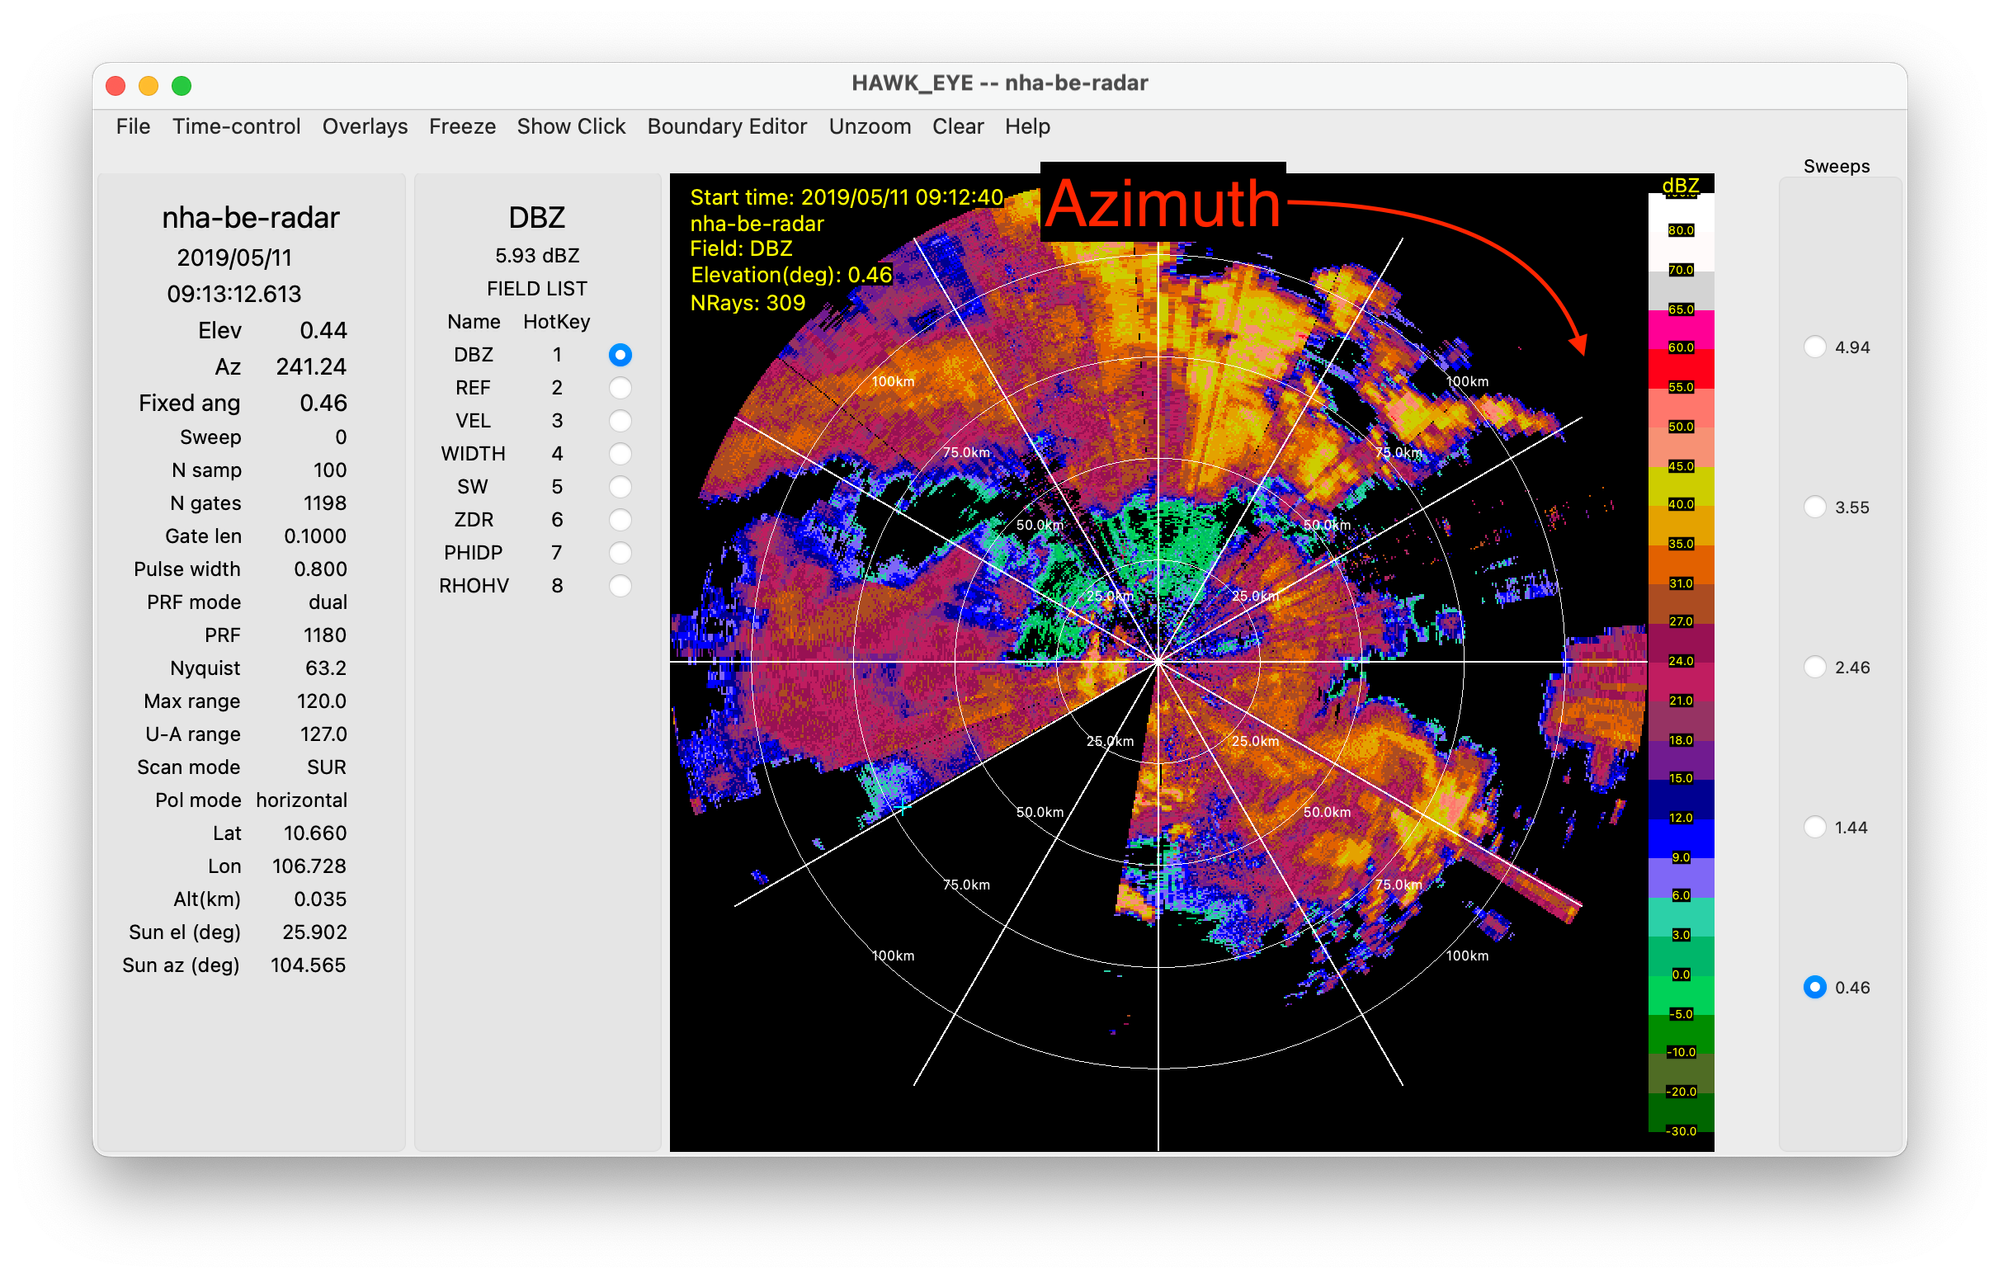
\includegraphics[width=0.8\textwidth]{Images/3.5-hawk-eye.png}
    \caption{HawkEye visualization tool}
    \label{fig:hawkeye}
\end{figure}